\documentclass{article}
\usepackage[UTF8]{ctex}
\usepackage{amsmath,mathtools,geometry,pgfplots,float,mathrsfs,caption,enumerate}
\pgfplotsset{compat=1.15}
\usetikzlibrary{arrows}
\geometry{scale=0.7}

\title{\vspace*{-3cm}\heiti 三角形练习\vspace{-1cm}}
\author{}
\date{}

\begin{document}
\maketitle
\begin{enumerate}
	\renewcommand{\labelenumi}{\textbf{\theenumi. }}
	\item 在$\mathrm{Rt}\triangle ABC$中, $\angle C=90^\circ$, $\angle B>\angle A$, $CD$是斜边上的高线,$CF$是斜边上的中线,$CE$是直角角平分线。请你判断$CD$, $CE$, $CF$的大小关系。
	\begin{figure}[H]
		\flushright
		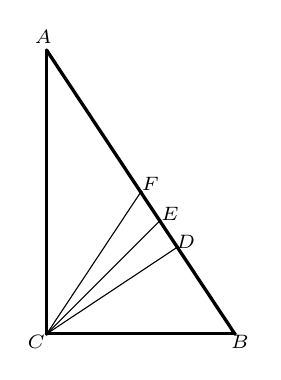
\begin{tikzpicture}[line cap=round,line join=round,>=triangle 45,x=1cm,y=1cm]
			\clip(-0.2420422812628917,-0.22932412271129332) rectangle (2.616022792551205,3.8882178331536);
			\draw [line width=1.2pt] (0.,3.5995517636730314)-- (2.388254453084374,0.);
			\draw [line width=1.2pt] (2.388254453084374,0.)-- (0.,0.);
			\draw [line width=1.2pt] (0.,0.)-- (0.,3.5995517636730314);
			\draw [line width=0.4pt] (0.,0.)-- (1.6582630221754502,1.1002353368171798);
			\draw [line width=0.4pt] (0.,0.)-- (1.4356920076406876,1.4356920076406876);
			\draw [line width=0.4pt] (1.194127226542187,1.7997758818365157)-- (0.,0.);
			\begin{scriptsize}
				\draw [fill=black] (0.,3.5995517636730314) circle (0.5pt);
				\draw[color=black] (-0.044783678710475824,3.7765367517802444) node {$A$};
				\draw [fill=black] (2.388254453084374,0.) circle (0.5pt);
				\draw[color=black] (2.4546374910425053,-0.1071039699102933) node {$B$};
				\draw [fill=black] (0.,0.) circle (0.5pt);
				\draw[color=black] (-0.13282591169590374,-0.1071039699102933) node {$C$};
				\draw [fill=black] (1.6582630221754502,1.1002353368171798) circle (0.5pt);
				\draw[color=black] (1.7649733326566537,1.16950840837841) node {$D$};
				\draw [fill=black] (1.4356920076406876,1.4356920076406876) circle (0.5pt);
				\draw[color=black] (1.5644326908565123,1.5265685754859784) node {$E$};
				\draw [fill=black] (1.194127226542187,1.7997758818365157) circle (0.5pt);
				\draw[color=black] (1.3149796973977999,1.9031936832569751) node {$F$};
			\end{scriptsize}
		\end{tikzpicture}
	\end{figure}
	\item 已知三角形的一边和这条边上的高线和中线, 求作这个三角形.
	\begin{figure}[H]
		\flushright
		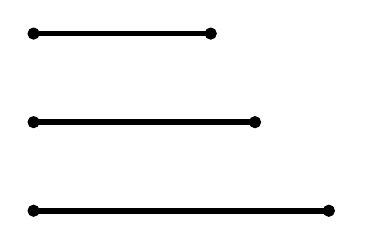
\begin{tikzpicture}[line cap=round,line join=round,>=triangle 45,x=0.75cm,y=0.75cm]
			\clip(-0.1,-0.1) rectangle (5.5,3.1);
			\draw [line width=2.pt] (0.,3.)-- (3.,3.);
			\draw [line width=2.pt] (3.75,1.5)-- (0.,1.5);
			\draw [line width=2.pt] (0.,0.)-- (5.,0.);
			\begin{scriptsize}
				\draw [fill=black] (0.,3.) circle (2.0pt);
				\draw [fill=black] (3.,3.) circle (2.0pt);
				\draw [fill=black] (0.,1.5) circle (2.0pt);
				\draw [fill=black] (3.75,1.5) circle (2.0pt);
				\draw [fill=black] (0.,0.) circle (2.0pt);
				\draw [fill=black] (5.,0.) circle (2.0pt);
			\end{scriptsize}
		\end{tikzpicture}
	\end{figure}
	\item 已知三角形的一角和这个角的角平分线以及这个角对边上的高,求作这个三角形.
	\begin{figure}[H]
		\flushright
		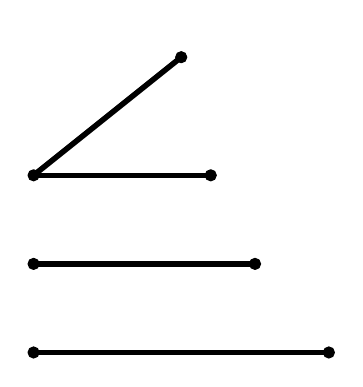
\begin{tikzpicture}[line cap=round,line join=round,>=triangle 45,x=0.75cm,y=0.75cm]
			\clip(-0.1,-0.1) rectangle (5.1,5.5);
			\draw [line width=2.pt] (0.,3.)-- (3.,3.);
			\draw [line width=2.pt] (3.75,1.5)-- (0.,1.5);
			\draw [line width=2.pt] (0.,0.)-- (5.,0.);
			\draw [line width=2.pt] (2.5,5.)-- (0.,3.);
			\begin{scriptsize}
				\draw [fill=black] (0.,3.) circle (2.0pt);
				\draw [fill=black] (3.,3.) circle (2.0pt);
				\draw [fill=black] (0.,1.5) circle (2.0pt);
				\draw [fill=black] (3.75,1.5) circle (2.0pt);
				\draw [fill=black] (0.,0.) circle (2.0pt);
				\draw [fill=black] (5.,0.) circle (2.0pt);
				\draw [fill=black] (2.5,5.) circle (2.0pt);
			\end{scriptsize}
		\end{tikzpicture}
	\end{figure}
	\item 已知三角形一条边上的高和中线, 以及另外一条边, 求作这个三角形.
	\begin{figure}[H]
		\flushright
		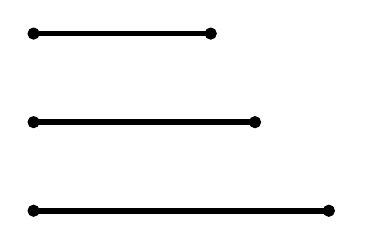
\begin{tikzpicture}[line cap=round,line join=round,>=triangle 45,x=0.75cm,y=0.75cm]
			\clip(-0.1,-0.1) rectangle (5.5,3.1);
			\draw [line width=2.pt] (0.,3.)-- (3.,3.);
			\draw [line width=2.pt] (3.75,1.5)-- (0.,1.5);
			\draw [line width=2.pt] (0.,0.)-- (5.,0.);
			\begin{scriptsize}
				\draw [fill=black] (0.,3.) circle (2.0pt);
				\draw [fill=black] (3.,3.) circle (2.0pt);
				\draw [fill=black] (0.,1.5) circle (2.0pt);
				\draw [fill=black] (3.75,1.5) circle (2.0pt);
				\draw [fill=black] (0.,0.) circle (2.0pt);
				\draw [fill=black] (5.,0.) circle (2.0pt);
			\end{scriptsize}
		\end{tikzpicture}
	\end{figure}
	\item 已知三角形的两边及第三边上的中线,求作这个三角形.
	\begin{figure}[H]
		\flushright
		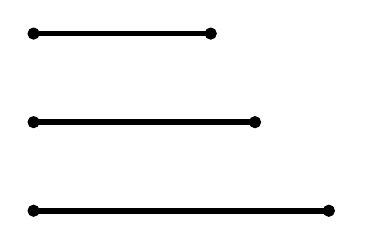
\begin{tikzpicture}[line cap=round,line join=round,>=triangle 45,x=0.75cm,y=0.75cm]
			\clip(-0.1,-0.1) rectangle (5.5,3.1);
			\draw [line width=2.pt] (0.,3.)-- (3.,3.);
			\draw [line width=2.pt] (3.75,1.5)-- (0.,1.5);
			\draw [line width=2.pt] (0.,0.)-- (5.,0.);
			\begin{scriptsize}
				\draw [fill=black] (0.,3.) circle (2.0pt);
				\draw [fill=black] (3.,3.) circle (2.0pt);
				\draw [fill=black] (0.,1.5) circle (2.0pt);
				\draw [fill=black] (3.75,1.5) circle (2.0pt);
				\draw [fill=black] (0.,0.) circle (2.0pt);
				\draw [fill=black] (5.,0.) circle (2.0pt);
			\end{scriptsize}
		\end{tikzpicture}
	\end{figure}
	\item 已知三角形的一条边与这条边上的高, 和另外一条边, 求作这个三角形.
	\begin{figure}[H]
		\flushright
		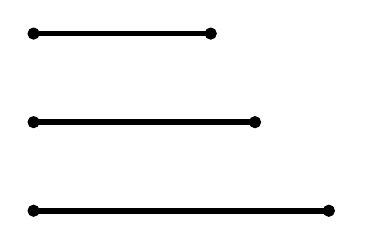
\begin{tikzpicture}[line cap=round,line join=round,>=triangle 45,x=0.75cm,y=0.75cm]
			\clip(-0.1,-0.1) rectangle (5.5,3.1);
			\draw [line width=2.pt] (0.,3.)-- (3.,3.);
			\draw [line width=2.pt] (3.75,1.5)-- (0.,1.5);
			\draw [line width=2.pt] (0.,0.)-- (5.,0.);
			\begin{scriptsize}
				\draw [fill=black] (0.,3.) circle (2.0pt);
				\draw [fill=black] (3.,3.) circle (2.0pt);
				\draw [fill=black] (0.,1.5) circle (2.0pt);
				\draw [fill=black] (3.75,1.5) circle (2.0pt);
				\draw [fill=black] (0.,0.) circle (2.0pt);
				\draw [fill=black] (5.,0.) circle (2.0pt);
			\end{scriptsize}
		\end{tikzpicture}
	\end{figure}
	\item 已知三角形的三条中线, 求作这个三角形.
	\begin{figure}[H]
		\flushright
		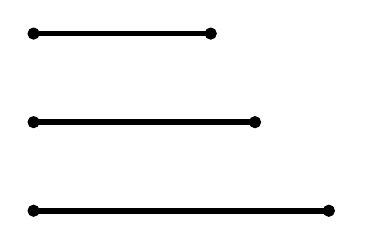
\begin{tikzpicture}[line cap=round,line join=round,>=triangle 45,x=0.75cm,y=0.75cm]
			\clip(-0.1,-0.1) rectangle (5.5,3.1);
			\draw [line width=2.pt] (0.,3.)-- (3.,3.);
			\draw [line width=2.pt] (3.75,1.5)-- (0.,1.5);
			\draw [line width=2.pt] (0.,0.)-- (5.,0.);
			\begin{scriptsize}
				\draw [fill=black] (0.,3.) circle (2.0pt);
				\draw [fill=black] (3.,3.) circle (2.0pt);
				\draw [fill=black] (0.,1.5) circle (2.0pt);
				\draw [fill=black] (3.75,1.5) circle (2.0pt);
				\draw [fill=black] (0.,0.) circle (2.0pt);
				\draw [fill=black] (5.,0.) circle (2.0pt);
			\end{scriptsize}
		\end{tikzpicture}
	\end{figure}
	\item (\kaishu 选做)\songti 已知三角形的三条高, 求作这个三角形.
	\begin{figure}[H]
		\flushright
		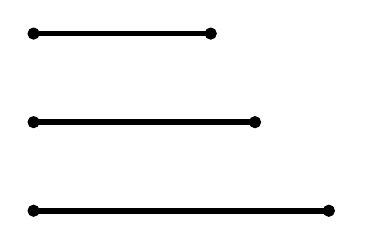
\begin{tikzpicture}[line cap=round,line join=round,>=triangle 45,x=0.75cm,y=0.75cm]
			\clip(-0.1,-0.1) rectangle (5.5,3.1);
			\draw [line width=2.pt] (0.,3.)-- (3.,3.);
			\draw [line width=2.pt] (3.75,1.5)-- (0.,1.5);
			\draw [line width=2.pt] (0.,0.)-- (5.,0.);
			\begin{scriptsize}
				\draw [fill=black] (0.,3.) circle (2.0pt);
				\draw [fill=black] (3.,3.) circle (2.0pt);
				\draw [fill=black] (0.,1.5) circle (2.0pt);
				\draw [fill=black] (3.75,1.5) circle (2.0pt);
				\draw [fill=black] (0.,0.) circle (2.0pt);
				\draw [fill=black] (5.,0.) circle (2.0pt);
			\end{scriptsize}
		\end{tikzpicture}
	\end{figure}

\end{enumerate}
\end{document}